\documentclass[twoside]{project}

\studnameA{Pedro Pérez Sánchez}
\studnameB{Juan Pablo Colomer}
\studuniA{pp2550}
\studuniB{jpc2192}
\coursename{Introduction to Computational Learning Theory}
\date{\today}
\begin{document}
\maketitle

\section*{Introduction}
The paper we studied is ``Knows What It Knows: A Framework For Self-Aware Learning''\cite{KWIK}.
This paper introduces a new learning framework called KWIK (Know What It Knows) that has some common elements with 
the learning frameworks covered in the course, PAC and OLMB.\\

This learning framework outputs a label only when it has certainty that is the correct label for the input given. Otherwise, it outputs
``I don't know`` ($\bot$). Additionally, there is a polynomial upper bound on the number of times a KWIK algorithm outputs $\bot$.\\

KWIK was motivated by the idea of distinguishing instances that have been learned with high accuracy from the others. \\

The structure of this document will be the following:
\begin{itemize}
  \item Section 2 provides a formal definition of the KWIK model. 
  \item Section 3 clarifies the definition of KWIK by using an example.
  \item Section 4 shows a set of concept classes that can be learned by a KWIK model.
\end{itemize}

\section*{Definition}
two


\section*{Clarifying example}
%Enhancement: Explain properly this algorithm as a KWIK algorithm
Let $G$ be a network graph with source $s$ and sink $t$ where every edge $(i,j)$ has a cost vector $v_{ij}$ associated to it. Let $w$ be a weight vector. The cost for an agent to traverse the edge $(i,j)$ is $cost(i,j)=w \cdot v_{ij}$. \\

The algorithm knows $G, v_{ij}$ for all edges $(i,j)$  and every time it traverses the edge $(i,j)$ it receives $w \cdot v_{ij}$. However, it doesn't know $w$.  \\

The goal of the algorithm is to find a path from source $s$ to sink $t$ with the lowest for the agent in the fewest possible attempts.

For the example on figure \ref{fig:sec2.1} assume $w=[1,2,0]$. There are three possible paths from $s$ to $t$.
\begin{itemize}
  \item The path $s\to c \to l \to t$ has a total cost of 3
  \item The path $s\to c \to t$ has a total cost of 4
  \item The path $s\to c \to a \to t$ has a total cost of 5
\end{itemize}

In the first attempt, a logical thing to do is to assume that $w$ is uniform. In other words $w = [q,q,q]$ with $q \in \mathbb{R}$. As a result, the agent will follow path $s\to c \to t$ because its predicted cost is the lowest. Then, it will receive $cost(s,c)=3$ and $cost(c,t)=1$  \\

By using linear algebra, the algorithm knows that 
\begin{align}
  [w_1,w_2,w_3]\cdot [1,1,1] &=  3 \nonumber\\
  w_1+w_2+w_3 &=  3 \label{eqn:sec2.1}\\
  \nonumber\\
  [w_1,w_2,w_3] \cdot [1,0,0] &= 1 \nonumber\\
  \Rightarrow w_1 &=  1 \label{eqn:sec2.2}
\end{align}

After getting this information, the algorithm needs to decide the next path it will follow. Additionally, the $cost(a,t)$ must be equal to $0$ because $v_{at} = [0,0,0]$ and the algorithm can deduce $cost(c,a)$.
\begin{eqnarray*}
  cost(c,a) &=&  w \cdot [0,1,1] \\
  &=&  w \cdot ([1,1,1] - [1,0,0]) \\
  &=&  w \cdot [1,1,1] - w \cdot [1,0,0] \\
  &=&  w \cdot [1,1,1] - w \cdot [1,0,0] \\
  &=&  cost(s,c) - cost(a,t) \\
  &=&  3 - 1 \\
  &=&  2
\end{eqnarray*}
Therefore, it knows that the total cost of path $s \to c \to a \to t$ is $5$ which is not the minimum path.
Given that $v_{cl}$ is linearly independent of $v_{sc},v_{ct}$ it's impossible for the algorithm to know $cost(c,l)$ with the current information. Hence, it knows it doesn't know the total cost of $s \to c \to l \to t$. \\

In order to gather unknown information, in the next attempt the agent traverses path $s \to c \to l \to t$. After this, it will receive $cost(c,l) = 0$.
\begin{eqnarray}
  [w_1,w_2,w_3] \cdot [0,0,1] &=& 0 \nonumber\\
  w_3 &=& 0 \label{eqn:sec2.3}
\end{eqnarray}

By using equations (\ref{eqn:sec2.1}), (\ref{eqn:sec2.2}), (\ref{eqn:sec2.3}) the algorithm calculates $w=[1,2,0]$.
Now it is certain that the path with minimum total cost is $s \to c \to l \to t$. \\

In every attempt, this algorithm will either take the optimal path or take a path that contains a cost vector which is linearly independent to all the cost vectors previously explored. In the general case, with cost vectors of dimension $d$, the algorithm only needs to traverse $d$ edges with linearly independent cost vectors. Consequently, the number of $\bot$s is upper bounded by $d$.


\section*{Some KWIK Learnable Classes}
In this section we will describe some concept classes that can be learned under
the KWIK model.

\paragraph{Algorithm 1: Memorization Algorithm}
Given a finite input space $X$ and noise-free observations, any concept class
can be learned under the KWIK model with a KWIK bound of $|X|$ by using the
memorization algorithm. Which, for every received example $x \in X$:
\begin{enumerate}
  \item If it is the first time it receives $x$, the algorithm outputs $\bot$,
  receives the correct label of $x$, and memorizes it.
  \item If it is not the first time it receives $x$, the algorithm has already
  memorized its correct label, so it outputs it.
\end{enumerate}

This algorithm will output $\bot$ at most once per example, because it is
impossible to see an example twice for the first time. Therefore, the KWIK bound
of the memorization algorithm is $|X|$. \\

\paragraph{Algorithm 2: Enumeration Algorithm}
Given any input space $X$ and noise-free observations, any finite concept class
can be learned under the KWIK model with a KWIK bound of $|C| - 1$ by using the
elimination algorithm. The elimination algorithm maintains a set of ``potential
target concepts'' $\hat{H}$, initialized as $C$. For every received example
$x \in X$, It creates a set $\hat{L} = \{ h(x) | h \in \hat{H} \}$ and:
\begin{enumerate}
  \item If $|\hat{L}| > 1$, it outputs $\bot$ because at least 2 hypotheses
  disagree in labeling $x$. When the correct label of $x$ is received, it
  updates $\hat{H}$ by eliminating from it all the hypotheses that
  misclassified $x$.
  \item If $|\hat{L}| = 1$, it outputs the element in $\hat{L}$.
  \item If $|\hat{L}| = 0$, it means that the target concept in use is not in
  the concept class being learned. This should never happen.
\end{enumerate}

For every $\bot$ that the algorithm returns, it will eliminate at least one
concept from $\hat{H}$. Initially, $|\hat{H}| = |C|$. If the target
concept belongs to $C$, at the end of its execution, the algorithm will have
eliminated $|C| - 1$ concepts from $\hat{H}$. Therefore, the maximum number
of $\bot$s that the algorithm will output is $|C| - 1$.

\paragraph{Example 1:} The PhD lounge is frequented by a set $S$ of $n$ CLT
students. Every two weeks, a subset of them $G \subseteq S$ meets there to work
together on an assignment from the class. One of the students $f \in S$ is an
expert in slowing down the entire group, and whenever he is in the PhD lounge
($f \in G$), all the students in $G$ are forced to ``pull an all-nighter''.
Fortunately, there is another student $p \in S$ who is a genius, and, whenever
he is in the PhD lounge ($p \in G$), everyone is able to finish on time and go
home early, independently on the presence/absence of $f$. Rocco heard about the
story, and he wants to predict whether a subset of the students will ``pull an
all-nighter'' or not. However, he doesn't know the identity of $f$ and $p$. \\

The input space $X$ is all the possible subsets of $S$ ($|X| = 2^n$). Moreover,
the concept class to learn are all the possible assignments of $p$ and $f$
($|C| = n(n - 1)$). Therefore:
\begin{itemize}
  \item The memorization algorithm would achieve a KWIK bound of $2^n$.
  \item The enumeration algorithm would achieve a KWIK bound of $n(n - 1) - 1$.
\end{itemize}

\begin{figure}
  \centering
  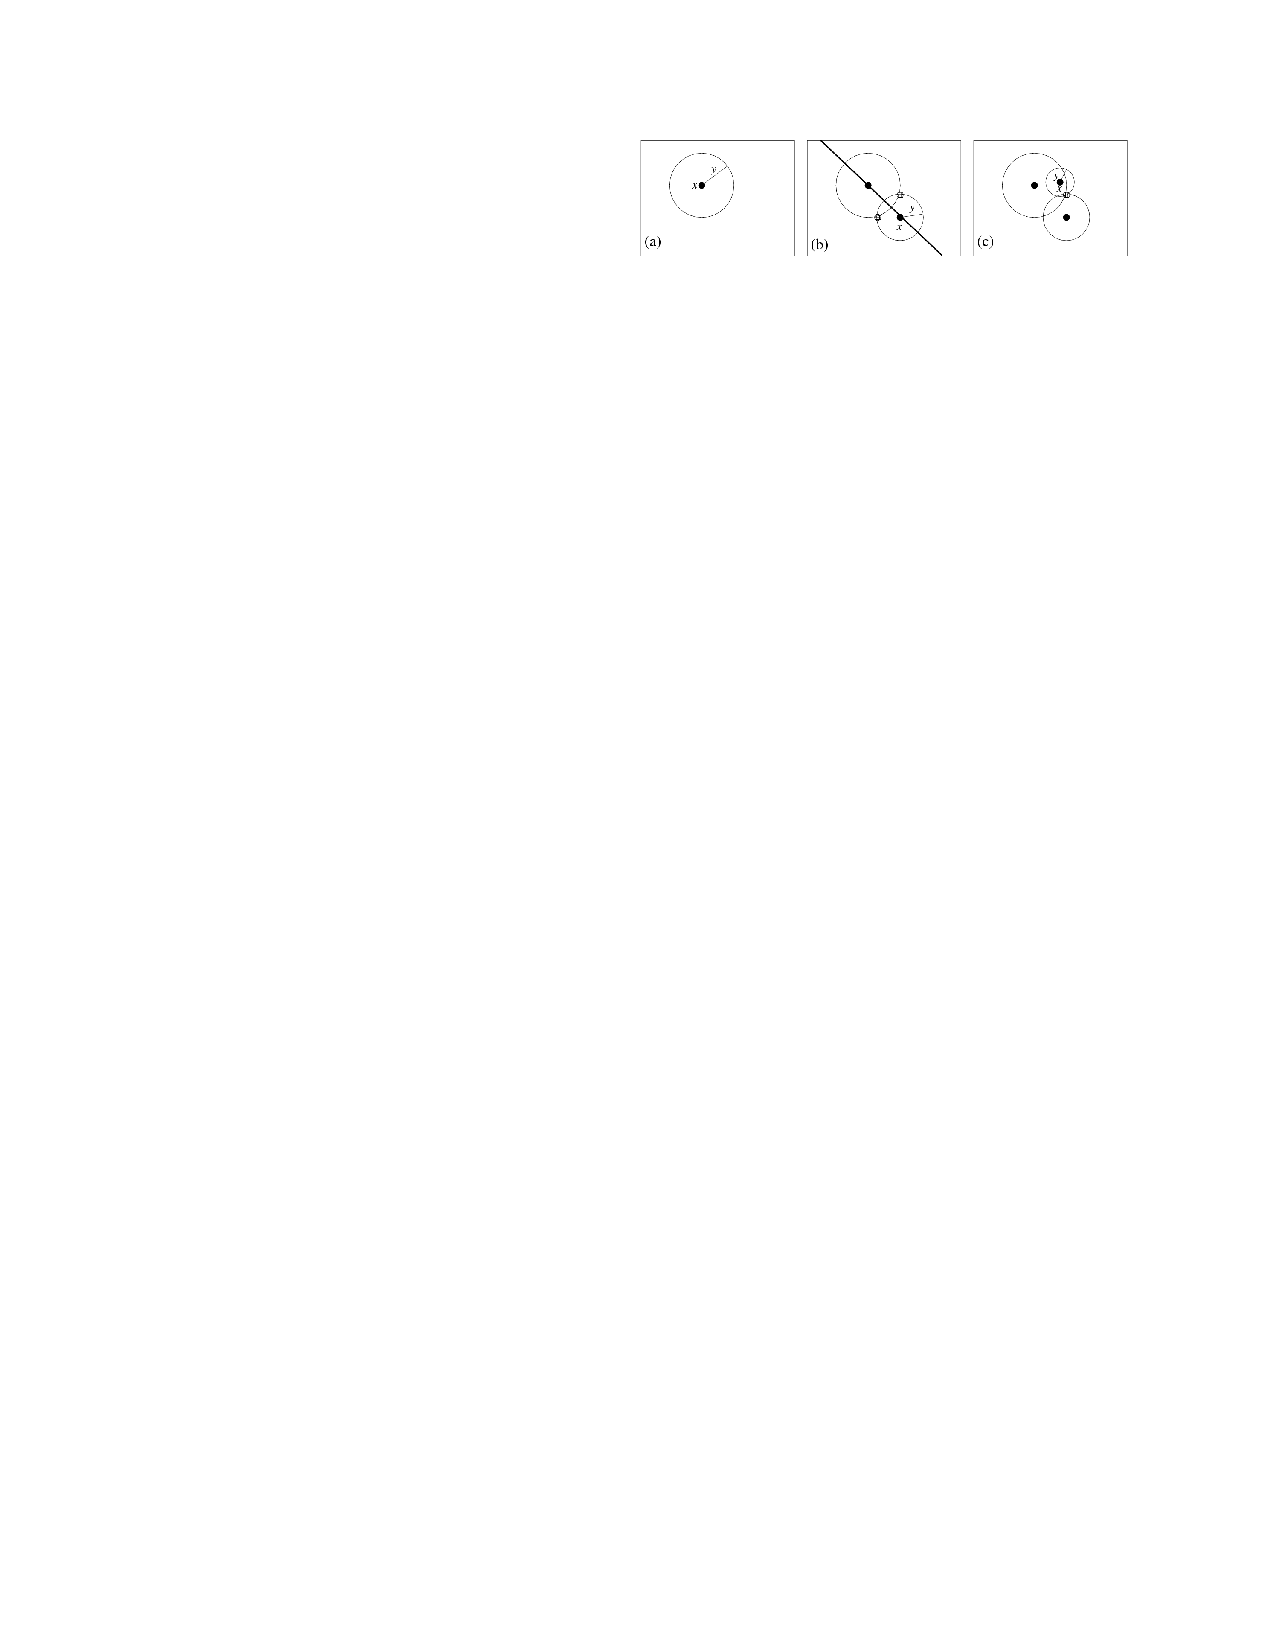
\includegraphics[width=0.5\textwidth]{figures/algorithm3.pdf}
  \label{fig:sec4.1}
  \caption{Planar-distance Algorithm \textcolor{red}{por ahora}}
\end{figure}

\paragraph{Algorithm 3: Planar-distance Algorithm}
The two algorithms described above are limited to learning a finite concept
class $C$ or receiving a finite input space $X$. In this algorithm, this
restriction doesn't exist. \\

Let:
\begin{itemize}
  \item $ X = \mathbb{R}^2 $
  \item $ Y = \mathbb{R} $
  \item $ C = \{ f \ | \ f : X \to Y, \hat{x} \in \mathbb{R}^2, f(x) = \norm{x - \hat{x}}_2 \} $
\end{itemize}

There is an unknown point $\overline{x}$ and the target concept $c(x)$ outputs
the distance between an example $x$ and point $\overline{x}$. \\
\begin{enumerate}
  \item For an initial input $x_1$, the algorithm outputs $\bot$ and it receives
  the output $y_1$. Now, the algorithm knows that $\overline{x}$ is in the
  circumference $c_1$, with radius $y_1$ centered at $x_1$.
  \item When the algorithm receives the second example $x_2$:
  \begin{itemize}
    \item If $x_2 = x_1$, it returns $y_1$.
    \item Otherwise, it returns $\bot$ and receives the output $y_2$. Similarly,
    the algorithm knows that $\overline{x}$ lies in the circumference $c_2$ with
    radius $y_2$ centered at $x_2$. Then, $\overline{x}$ is restricted to one of
    the two intersecting points ($i_1$ and $i_2$) of $c_1$ and $c_2$, as illustrated in Figure
    \ref{fig:sec4.1} (b). At this point, if $c_1$ and $c_2$ are tangent, $i_1 =
    i_2 = \overline{x}$.
  \end{itemize}
  \item When the algorithm receives the third example $x_3$:
  \begin{itemize}
    \item If $x_3$ is collinear with $x_1$ and $x_2$, then, $\norm{x_3 - i_1} =
    \norm{x_3 - i_2}$. So, it returns $\norm{x_3 - i_1}$.
    \item If it is not collinear, then it returns $\bot$ and receives the output
    $y_3$. Similarly, the algorithm knows that $\overline{x}$ lies in the
    circumference $c_3$ with radius $y_3$ centered at $x_3$. Now, circumferences
    $c_1$, $c_2$ and $c_3$ only have one intersecting point, which is
    $\overline{x}$.
  \end{itemize}
\end{enumerate}

We just showed that, for any input set, the algorithm will completely identify
$\overline{x}$ by outputting at most $3 \bot$s. Therefore, the KWIK bound of the
planar-distance algorithm is $3$. As we saw in the case of $x_3$ being collinear
with $x_1$ and $x_2$, there are instances in which a KWIK algorithm can
have enough information for returning valid answers before having learned the
target concept.

\paragraph{Algorithm 4: Coin-Learning Algorithm}
We will now consider a simple KWIK algorithm which learns the probability of a
biased coin to come up heads. This algorithm will receive Bernoulli observations
($0$ when the coin comes up tails and $1$ when it comes up heads) and, with a
KWIK bound of $B(\varepsilon, \delta) = O(frac{1}{\varepsilon^2}\log \frac{1}{\delta})$, it learns the
bias $p$ of the coin with $\varepsilon$-accuracy with probability at least $1-\delta$.

Let $\hat{p}$ be the estimate of $p$ made by the algorithm. It wants to estimate
the probability so that $|\hat{p} - p| \leq \varepsilon$.


Let $T$ be the number of observations it needs in order to satisfy the $\varepsilon$ and $\delta$ requirements.
Let $z_i$ be the $i$-th observation received by the algorithm.

\begin{itemize}
  \item If $i < T$ the algorithm can't guarantee that it will
  output an $\varepsilon$-accurate estimate with confidence $1-\delta$.
  \item Otherwise it calculates and outputs $\hat{p} = \frac{1}{T}\sum_{t=1}^{T}z_t$.
\end{itemize}
$T$ can be calculated by using a Hoeffding bound
\begin{eqnarray*}
  Pr[\hat{p} - p \geq \varepsilon] &\leq&  e^{-2T\varepsilon^2} \leq \delta/2 \\
  e^{-2T\varepsilon^2} &\leq& \delta/2 \\
  \Rightarrow T &\geq& \frac{1}{2\varepsilon^2}\ln \frac{2}{\delta}
\end{eqnarray*}

\begin{eqnarray*}
  Pr[\hat{p} - p \leq -\varepsilon] &\leq&  e^{-2T\varepsilon^2} \leq \delta/2 \\
  e^{-2T\varepsilon^2} &\leq& \delta/2 \\
  \Rightarrow T &\geq& \frac{1}{2\varepsilon^2}\ln \frac{2}{\delta}
\end{eqnarray*}

If $T = \frac{1}{2\varepsilon^2}\ln \frac{2}{\delta}$, with probability at least
$1 - \delta$, the algorithm will return an estimate $\hat{p}$ such that
$|\hat{p} - p| \leq \varepsilon$.

\paragraph{Algorithm 5: Noisy Linear-Regression Algorithm}
In section 3, we saw an algorithm for learning a weight vector $w$ such that
$f(x) = w \cdot x \ \forall x \in X$. In that case, what we observed was the
true value of $w \cdot x$. However, in the presence of additive noise, we don't
observe the true value, instead, we receive $w \cdot x + \eta$, with $\eta$
being the noise. This problem was solved by Stehl and Littman (2008)
\cite{Strehl}. The KWIK bound for this algorithm is $B(\varepsilon, \delta) =
O\left( \frac{d^3}{\varepsilon^4} \right)$, where $w \in \mathbb{R}^d$.


\section*{}
% TODO: Rename H to C

In this section, we will present a set of algorithms that, by combining KWIK
learners, are able to learn a more complex concept class. \\

\paragraph{Algorithm 6: Union Algorithm}
Let $H_i: X \to Y$ be a KWIK-learnable concept class by an algorithm $A_i$
with KWIK bound of $B_i(\varepsilon, \delta)$ for $1 \leq i \leq k$. Note that
all $H_1, \ldots, H_k$ share the same input and output spaces. \\

The union algorithm learns $H = \bigcup_i H_i$ with KWIK bound $B(\varepsilon,
\delta) = (k - 1) + \sum_{i = 1}^k B_i(\varepsilon, \delta)$. This can be
understood as a generalization of the Enumeration Algorithm (Algorithm 2). \\

The union algorithm maintains a set of ``potential algorithms'' $\hat{A}$,
initialized as $\{ A_1, \ldots, A_k \}$. For every received example
$x \in X$, it runs all algorithms in $\hat{A}$ to obtain a prediction from each
of them $\hat{y}_i$. It creates a set $\hat{L} = \{ \hat{y}_i | A_i \in \hat{A} \}$:
\begin{enumerate}
  \item If $\bot \in \hat{L}$, at least one of the algorithms doesn't know the
  answer with enough accuracy, then the union algorithm outputs $\bot$ and, once
  the correct label is received, it passes it to each of the algorithms that
  returned $\bot$.
  \item If $|\hat{L}| > 1$, at least two algorithms disagree on labeling $x$.
  Then, the union algorithm outputs $\bot$. Once the correct label $y$ is
  received, it eliminates from $\hat{A}$ the algorithms for which $\hat{y}_i(x)
  \neq y$.
  \item Otherwise, $|hat{L}| = 1$. This means that all the algorithms in
  $\hat{A}$ agree on labeling $x$. The union algorithm outputs the label in
  $\hat{L}$.
\end{enumerate}

The algorithm will only output $\bot$ in the first or second cases described
above:
\begin{itemize}
  \item In the first case, the algorithm will output at most $\sum_{i = 1}^k
  B_i(\varepsilon, \delta)$.
  \item In the second case, the union algorithm is going to eliminate at least one
  algorithm from $\hat{A}$. Initially, $|\hat{A}| = k$, so the algorithm will
  output $\bot$ at most $k - 1$ times and eliminates $k - 1$ algorithms from
  $\hat{A}$.
\end{itemize}

In total, the KWIK bound of the union algorithm is the sum of both cases:
$$ B(\varepsilon, \delta) = (k - 1) + \sum_{i = 1}^k B_i(\varepsilon, \delta) $$


\paragraph{Example 2}
Let:
\begin{itemize}
  \item $X = Y = \mathbb{R}$
  \item $H_1 = \{ f \ | \ f(x) =|x - c|, c \in \mathbb{R} \}$ KWIK learnable by $A_1$
  \item $H_2 = \{ f \ | \ f(x) = mx + b, m \in \mathbb{R}, b \in \mathbb{R} \}$ KWIK learnable by $A_2$
  \item $H = H_1 \cup H_2$
\end{itemize}

$H_1$ can be learned using a 1 dimension version of Planar-distance Algorithm (Algorithm 3) with a
KWIK bound of 2. $H_2$ can be learned with a KWIK bound of $2$,
the number of points needed to define a line.
$H$ is KWIK learnable using the union algorithm.
\begin{enumerate}
  \item Initially, $\hat{A} = \{A_1, A_2 \}$
  \item First, the algorithm receives $x_1 = 2$. $\hat{L} = \{ \bot \}$ because none of the algorithms knows the answer. Then, it outputs $\bot$ and receives $y_1 = 2$, which it passes to $A_1$, $A_2$.
  \item The algorithm receives $x_2 = 8$. $A_1$ and $A_2$ still don't know the actual value. Therefore, $\hat{L} = \{ \bot \}$ and it outputs $\bot$. Afterwards, it receives and passes $y_2 = 4$ to $A_1$ and $A_2$.
    Since $A_1$ and $A_2$ have returned $\bot$ twice, they have learned an hypothesis for every $x \in \mathbb{R}$.
    \begin{itemize}
      \item $A_1$ knows that $c = 4$. Because it's the only point that has a distance of $2$ from $x_1=2$ and 4 from $x_2 = 8$.
      \item $A_2$ learns the line that connects $(x_1, y_1)$ and $(x_2, y_2)$. Therefore, $m = 1/3$ and $b = 4/3$.
    \end{itemize}
  \item The algorithm receives $x_3 = 1$. $\hat{L} = \{ 3, 5/3 \}$
    \begin{itemize}
      \item $A_1$ predicts $3$
      \item $A_2$ predicts $5/3$
    \end{itemize}
    It returns $\bot$ because $A_1$ and $A_2$ disagree. Then it receives $y_3 = 3$ and eliminates algorithm $A_2$.
    From now on the algorithm will predict all the examples using $A_1$.
\end{enumerate}

\paragraph{Algorithm 7: Input-Partition Algorithm}
Let:
\begin{itemize}
  \item $X = \bigcup_{i=1}^k X_i$, where all $X_i \cap X_j = \emptyset \forall i \neq j$
  \item $H_i: X_i \to Y$ be a KWIK-learnable concept class by an algorithm $A_i$
  with KWIK bound of $B_i(\varepsilon, \delta)$ for $1 \leq i \leq k$. Note
  that all $H_1, \ldots, H_k$ share the same output space but their input spaces
  are disjoint.
  \item $H \subseteq X \to Y$ be a concept class.
\end{itemize}

The input-partition algorithm KWIK-learns $H$ with KWIK bound $B(\varepsilon,
\delta) = \sum_{i=1}^k B_i(\varepsilon, \delta/k)$. \\

When the algorithm receives an $x \in X_i$, it calls $A_i$ with parameters
$\varepsilon$ and $\delta/k$ and returns its response. By definition of $A_i$,
its response will be $\varepsilon$-accurate with probability at least $1 -
\delta/k$. Using union bounds, we know that the response over all $X$ of the
algorithm will be $\varepsilon$-accurate with probability at least $1 - \delta$.
Given that $X$ is the union of $k$ disjoint input spaces, the KWIK bound
of the input-partition algorithm will be $B(\varepsilon, \delta) = \sum_{i=1}^k
= (\varepsilon, \delta/k)$.

\paragraph{Example 3} Let $G$ be a Markov Decision Process consisting of $n$
states and $m$ actions. There are $n^2m$ transitions represented as triplets of
the form $(state_{origin}, action, state_{target})$. We want to learn the
probability of each transition to happen. By receiving Bernoulli observations,
we can KWIK-learn this using algorithm 7 (Input-Partition Algorithm) which
uses algorithm 4 (Coin-Learning Algorithm) as its $A_i$ for every $1 \leq i \leq
n^2m$ with parameters $\varepsilon$ and $\frac{\delta}{n^2m}$. The KWIK bound of
this algorithm is $B(\varepsilon, \delta) = n^2m \cdot O(\frac{1}{\varepsilon^2}
\ln \frac{n^2m}{\delta}) = O(\frac{n^2m}{\varepsilon^2} \ln \frac{nm}{\delta})$.

\paragraph{Algorithm 8: Cross-Product Algorithm}
Let
\begin{itemize}
  \item $H_i \subseteq X_i \to Y_i$ be a KWIK learnable concept class with bound $B_i(\varepsilon, \delta)$
\end{itemize}



\bibliography{library}{}
\bibliographystyle{plain}

\end{document}
